Consider the question ``Is there a correlation between the population of a country and its Gross Domestic Product (GDP)?''. The data for population and GDP can only be obtained independently from different sources. Suppose each data set is a relation. To apply visualization or analysis techniques to the data, the two relations must first be joined such that each row in the resulting relation represents a country and contains values for both population and GDP.

Integrating data from a variety of independent sources makes the data more useful, informative, and valuable for visualization and analysis tasks. Existing data integration and multidimensional analysis approaches typically target relational data sources. The data cube concept from the area of Online Analytical Processing (OLAP) is suitable for modeling statistical data sets. These approaches do not readily support integration of pre-computed data cubes, which is applicable for primarily scientific and social data analysis and visualization.

There is immense potential value in data that is not being realized. While publicly available data sets for just about any topic are published on the Web, it is difficult to realize their full value in practice because they exist in many different formats and vocabularies. The heterogeneity of these formats and vocabularies also makes it difficult to combine and analyze these data sets, and hinders the development of general purpose visualization tools.

This chapter presents novel data structures and algorithms for data set representation, integration and querying based on the data cube concept. The proposed framework is called the Universal Data Cube (UDC). Using this approach, many data sources can be integrated together into a single data structure. General purpose data visualization and analysis tools can then operate by querying the integrated data structure. Figure \ref{fig:flow} shows the overall flow enabled by the UDC, from disparate data sets to general purpose interactive visualizations.

\begin{figure}
  \centering
  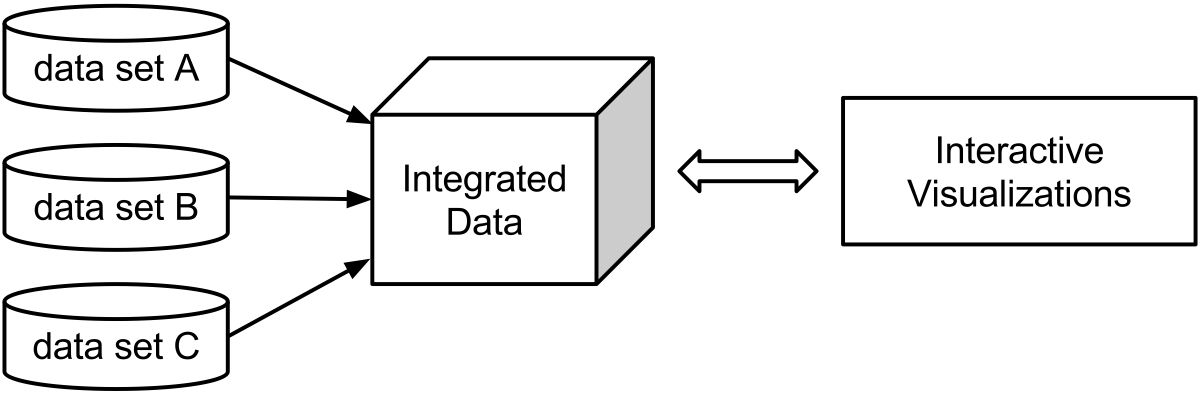
\includegraphics[width=\figureWidth]{figs/flow.png}
  \caption [Universal Data Cube Overview]{The overall context of the UDC as a technology for data integration for the purpose of interactive visualization. }
  \label{fig:flow}
\end{figure}

\section{Related Work}
Existing approaches to representing, visualizing, and analyzing are vast. The relational model is the foundation of relational databases. Data cubes are multidimensional aggregated relations suitable for visualization and analysis. The field of knowledge management is concerned with general data models representing vast collections of concepts and facts. Data integration is an area focusing on techniques for combining data from many sources.

Relational database systems provide a mature data management solution and are widely adopted \cite{ramakrishnan2000database}. Relational algebra is the theoretical underpinning of relational databases \cite{clifford1985algebra}. Perhaps the most familiar data representation system today is the spreadsheet, which is capable of representing relations as well as complex operations across data values \cite{eick2000visualizing}. Many organizations use spreadsheets, employing Microsoft Excel, Google Docs, or other tools to manage data or make data available. For example, the United Nations Department of Economic and Social Affairs provides their population statistics in Excel format (see figure \ref{fig:unPopExcel}).

The term ``data cube'' was originally introduced as a relational operator generalizing group-by, cross-tab, and sub-totals \cite{gray1997data}. The data cube operator produces relations containing aggregated values from other relations. Data warehouse systems are typically built on the relational model and are augmented by data cubes, also known as OLAP (OnLine Analytical Processing) cubes, for reporting and analysis \cite{codd1993providing}. The term OLAP stands in contrast to OLTP (OnLine Transaction Processing), which is the part of the data warehouse system that ingests and stores data at the level of individual transactions or events. After the ETL (Extract, Transform and Load) phase of the data warehouse flow, the data is analyzed by computing a data cube from the transactional data.

Data cubes contain summaries of the collection of facts stored in a relational database \cite{chaudhuri1997overview}. For example, a data cube may contain how much profit was made from month to month subdivided by product category, while the relational database may contain the information associated with each individual transaction. Because data cubes provide a higher level of abstraction, they are a widely used method of data abstraction for supporting visualization and analysis tasks. Kimball pioneered the area of ``Dimensional Modeling,'' which concerns constructing data warehouse schemas amenable to OLAP-based analysis \cite{kimball1998data}. Data cubes have been implemented in a variety of different systems, so effort has been made to discover unified conceptual or mathematical models that can characterize many implementations \cite{datta1999cube, vassiliadis1999survey, vassiliadis1998modeling, li1996data, agrawal1997modeling, gyssens1997foundation, blaschka1998finding}.

The data cube concept and structure can be used to model existing data as well. Publicly available data sets (often termed ``statistical data'') may be considered as pre-computed data cubes if they contain aggregated measures (also called ``indicators,'' ``metrics,'' or ``statistics'') across time, geographic space, and other dimensions such as gender, age range, ethnicity, religion, or industry sector.

Existing OLAP technologies assume that the data cubes will be computed from a relational source. They are not designed to handle integration of pre-computed data cubes that may use inconsistent identifiers for common dimensions and measures between multiple data sets. Therefore, the application of the data cube concept to integration and visualization of many pre-computed data cubes, while theoretically plausible, requires the development of novel data structures and algorithms that extend the data cube model to handle integration of pre-computed data cubes that may use inconsistent identifiers for common dimensions and measures. With this approach, it is possible to model many data sets using their shared dimensions and measures. This enables integration of many data sets into a single structure suitable for visualization and analysis.

The Semantic Web is a vision of a ``Web of Data'' coexisting with the World Wide Web \cite{berners2001semantic}. The basis of the Semantic Web is the Resource Description Framework (RDF) data model, which represents a graph of data in the form of $(subject, predicate, object)$ triples. The Semantic Web vision has evolved into the concept of Linked Data, which refers to data that is available as RDF and made available according to common conventions \cite{bizer2009linked, bizer2007publish}. Any data that can be represented using a relational database can also be represented using RDF \cite{bizer2006d2r}. The SPARQL query language for RDF can be used to query and integrate data from multiple sources \cite{quilitz2008querying}. Lopez et al.\ developed an information management system for integrating and analyzing heterogeneous information sources characterizing urban areas \cite{lopez2012queriocity}. The Semantic Web technology stack contains a method for declaring when different identifiers refer to the same entity and processing queries appropriately to integrate data \cite{halpin2010owl, ding2010sameas}. While the Semantic Web provides a compelling vision, its adoption is not as widespread as one might expect \cite{lytras2008semantic}.

The RDF Data Cube Vocabulary is capable of representing data cubes using Semantic Web technologies \cite{rdfdatacube}. The intention of the RDF Data Cube Vocabulary is to provide a common representation and interchange format for statistical data. The RDF Data Cube Vocabulary draws from a previous effort called the Statistical Data and Metadata eXchange (SDMX) initiative that was launched in 2001 by seven organizations working on statistics at the international level \cite{cyganiak2010semantic}. The primary challenges faced when using the RDF Data Cube Vocabulary include transforming to and from well known formats and data models. Salas et al.\ discussed how data can be transformed from existing OLAP systems or flat files into RDF using the Data Cube Vocabulary and introduced a faceted visualization tool for RDF data cubes \cite{salas-icsc-2012}. K{\"a}mpgen et al.\ investigated how data represented using the RDF Data Cube Vocabulary can be transformed for analysis using traditional OLAP systems \cite{kampgen2011transforming}. Maali et al.\ proposed a pipeline for converting government data into high quality Linked Data utilizing the Data Cube Vocabulary \cite{maali2012publishing}.

The field of data integration offers many techniques for combining data from multiple sources based on the relational model \cite{doan2012principles} as well as from a theoretical perspective \cite{lenzerini2002data, halevy2006data, ziegler2004three}. Schema matching is the area of data integration that concerns semantic matching between the attributes of data tables from different sources \cite{rahm2001survey, fagin2003data}.

Schema matching may be performed manually, but it must be automated to scale to hundreds or thousands of different sources. Numerous approaches for automated schema matching have been proposed \cite{shvaiko2005survey, doan2001reconciling, kang2003schema, milo1998using, madhavan2001generic, doan2000learning}. Schema matching approaches aimed specifically at Web- and Ontology-based data integration have also been proposed \cite{he2003statistical, noy2004semantic, doan2005semantic, madhavan2007web, kalfoglou2003ontology, noy2009ontology, uschold2004ontologies, wache2001ontology, noy2003prompt, euzenat2007ontology}.

Data matching (also known as record linkage) is the area of data integration focusing on resolving different identifiers to the same real-world entity \cite{winkler1999state, winkler2006overview, koudas2006record, aizawa2005fast, gu2003record}. Record linkage has been applied extensively to public data \cite{jaro1995probabilistic, jaro1989advances, holman1999population}. Several tools have been introduced that aid users in data integration tasks via a graphical user interface \cite{christen2008febrl, kandel2011wrangler, elfeky2002tailor, gonzalez2010google}. Techniques from both of these areas must be applied to integrate data sets from multiple sources and use the proposed unified data model.

\section{Case Study: Causes of Death}
The Centers for Disease Control provides data on causes of death in the US over time. This data set was targeted for visualization as a case study in visualizing public data sets containing pre-aggregated data cubes. A natural way to visualize this data is as a stacked area chart, shown in figure \ref{fig:mortalityVisV2}. The table contained a hierarchy of diseases, and all but the top-level disease categories were removed manually. Selecting the subtree of causes of death to include in the visualization is one example of a task that would be automated with our data representation framework. Next, a JavaScript program was written that pivoted the table from a format where each column was a year to a format where each row is a year, making the table usable by D3.js. This table contained an entry for ``all causes,'' which was removed manually because it was not appropriate to include visualize.

The mortality data set was published in GitHub Pages using JavaScript Object Notation (JSON) \cite{crockford2006application} compatible with the structure accepted by D3 \cite{d3}. AMD (Asynchronous Module Definition) is a JavaScript pattern for publishing and consuming reusable modules across domains \cite{osmani2012learning}. The mortality data set was published as an AMD module containing JSON data rather than as a CSV or JSON file in order to circumvent the same-origin policy. This allows any Web page to consume the data set, not only pages within the same domain. This method of publishing was chosen because it is a simple way to publish data publicly with zero cost (as GitHub Pages is a free service for Open Source code), longevity, as GitHub is less likely to go offline in the future than a private server, and cross-domain availability (any page can load the module using an AMD loader such as \verb1require.js1). This method of publishing data is also developer-friendly, as most modern developers are familiar with GitHub.

The mortality stacked area visualization highlights several issues that must be addressed when using our proposed data representation framework. The causes of death extracted from the raw data are sometimes too long to use in the visualization as labels due to limited screen real estate. For example, ``Symptoms, signs, and abnormal clinical and laboratory findings, not elsewhere classified'' is too long to be placed next to its corresponding color in the legend of the visualization, and could be simplified to ``Unclassified conditions.'' In a data cube model, causes of death would be members in a dimension hierarchy. The labeling issue encountered in the mortality visualization indicates a need to support renaming of members for use as textual elements within visualizations. Since each label refers to a dimension member which may also be a generally well-known concept, the labels on the visualization could, for example, be links to the Wikipedia pages about the various causes of death, such as Cardiovascular Disease. In addition, there are 24 causes of death presented in this visualization using different colors, while the color scales provided by D3 and the color scale library ColorBrewer only support up to 20 colors. This issue indicates that it may be useful to be able to aggregate dimension members automatically as a new ``Other'' category in certain cases, or allow users to manually select only a subtree of a dimension hierarchy for visualization.

\begin{figure}[h!]
  \centering
  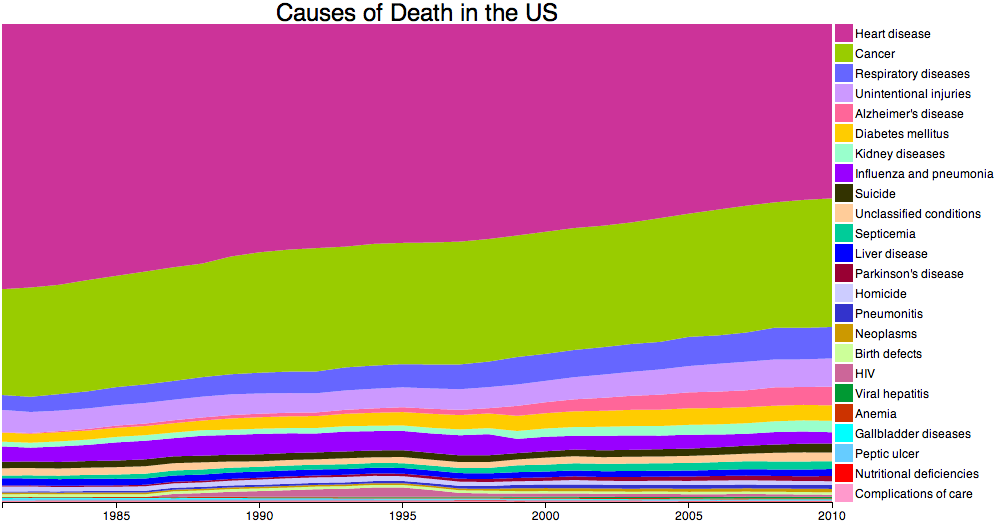
\includegraphics[width=\figureWidth]{figs/mortalityVisV2.png}
  \caption[CDC Mortality Visualization Version 2.]
   {A second pass at a stacked area visualization of Mortality data from the US Centers for Disease Control. This version has 25 hand-picked distinguishable colors, a color legend to spread out labels, and shortened labels in some cases.}
  \label{fig:mortalityVisV2}
\end{figure}

Figure \ref{fig:cardiovascularDiseaseRawTree} shows a sample of the raw data from which the hierarchy of causes of death must be gleaned. In this data, the hierarchy is encoded as an indented tree. Two different characters are used as indentation characters, ASCII codes 32 (space) and 65533 (unknown character). The level of indentation does not use a consistent number of indentation characters per indentation level. For example, the indentation level jumps from 0 to 4 to 7 to 10 to 13. We implemented an algorithm that parses the tree structure from an indented list and outputs the tree in the JSON structure compatible with D3.js hierarchical layouts. The JSON that the D3 Tree Layout algorithm expects is a tree data structure in which each node has a name and an array of child nodes. Leaf nodes may have additional quantitative properties to be visualized \cite{d3TreeLayout}.

Several D3 examples were drawn from to implement the cause of death tree visualization shown in figure \ref{fig:mortalityVisTree}, which uses the Reingold–Tilford ``tidy'' tree layout algorithm \cite{reingold1981tidier}. This visualization shows only the hierarchy of causes of death. No numerical values are associated with each node. Notice that the two causes of death that show the highest percentages in our stacked area visualization, Cancer and Cardiovascular Diseases, are the two nodes in the hierarchy that have the two largest subtrees of categorization.

The node-link tree visualization in figure \ref{fig:mortalityVisTree} demonstrates a visualization technique that can be applied to visualize dimension hierarchies in general. This implementation shows the structure of the hierarchy clearly, but has several drawbacks. Due to the size of the hierarchy, the inclusion of labels for all nodes necessitates small labels that are only legible at high resolution. When a hierarchy scales above certain thresholds of width and depth, this visualization becomes unwieldy, and labels must be truncated or omitted entirely. This is one example of the scalability issues that must be addressed when developing general-purpose visualization techniques.

\begin{figure}
  \centering
  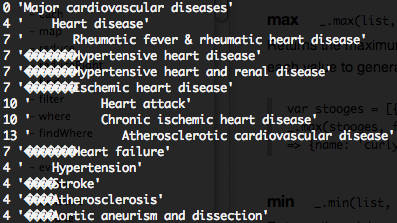
\includegraphics[width=\figureWidth]{figs/cardiovascularDiseaseRawTree.png}
  \caption[Cardiovascular disease raw tree.]
   {A portion of the raw data from the Centers for Disease Control encoding the hierarchy of causes of death. The number of indentation characters is shown on the left, and the content of the ``Cause'' field from the original CSV file is shown on the right in quotes. Note that there are two different indentation characters used, and the indentation level is not of a consistent multiple. This is one example of an unconventional format that must be parsed into a dimension hierarchy for use within our data representation framework.}
  \label{fig:cardiovascularDiseaseRawTree}
\end{figure}

\begin{figure}
  \centering
  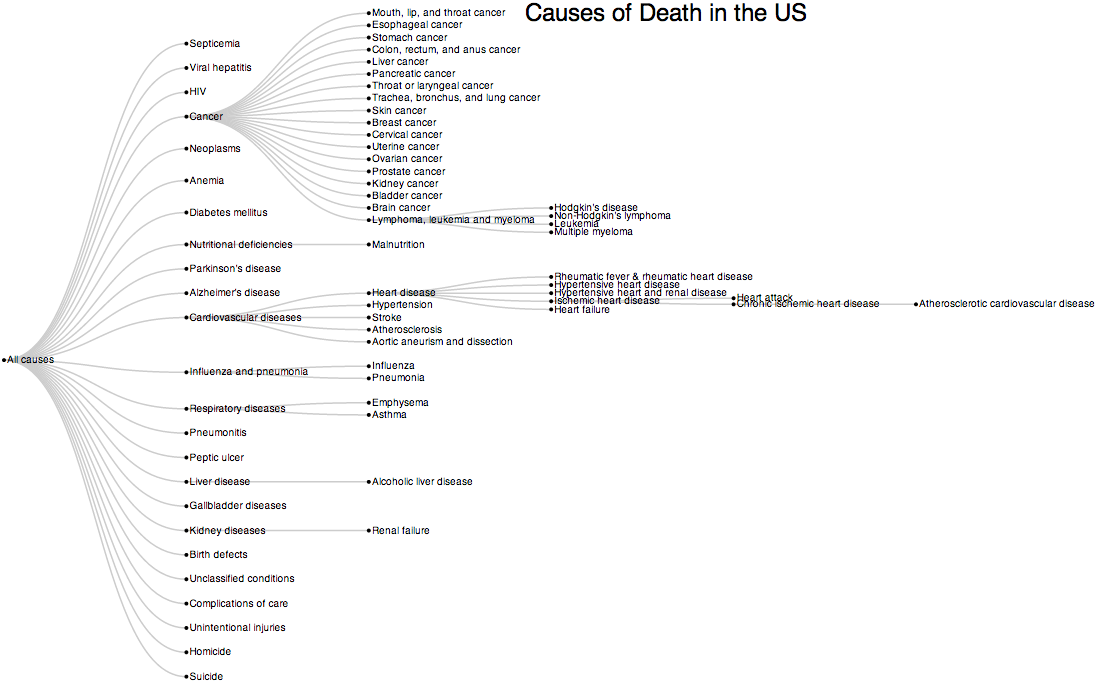
\includegraphics[width=\figureWidth]{figs/mortalityVisTree.png}
  \caption[Cause of Death Tree Visualization.]
   {A tree visualization of data from the Centers for Disease Control showing the hierarchy of causes of death. This is one example of a visualization that shows the structure of a dimension hierarchy.}
  \label{fig:mortalityVisTree}
\end{figure}

The pair of visualizations shown in figure \ref{fig:mortalityVisV4} is an example of a visualization dashboard with multiple linked views. The tree view shows a single level subtree. Black nodes have children, while white nodes do not. Clicking a black node causes the tree to drill down into the subtree with the clicked node as its root. When this interaction is executed, the stacked area visualization is recomputed to show the new set of disease causes that corresponds to the children of the newly selected node. In this way, the tree visualization provides interactions for drill down and roll up that define the slice of data shown in the stacked area chart.

\begin{figure}
  \centering
  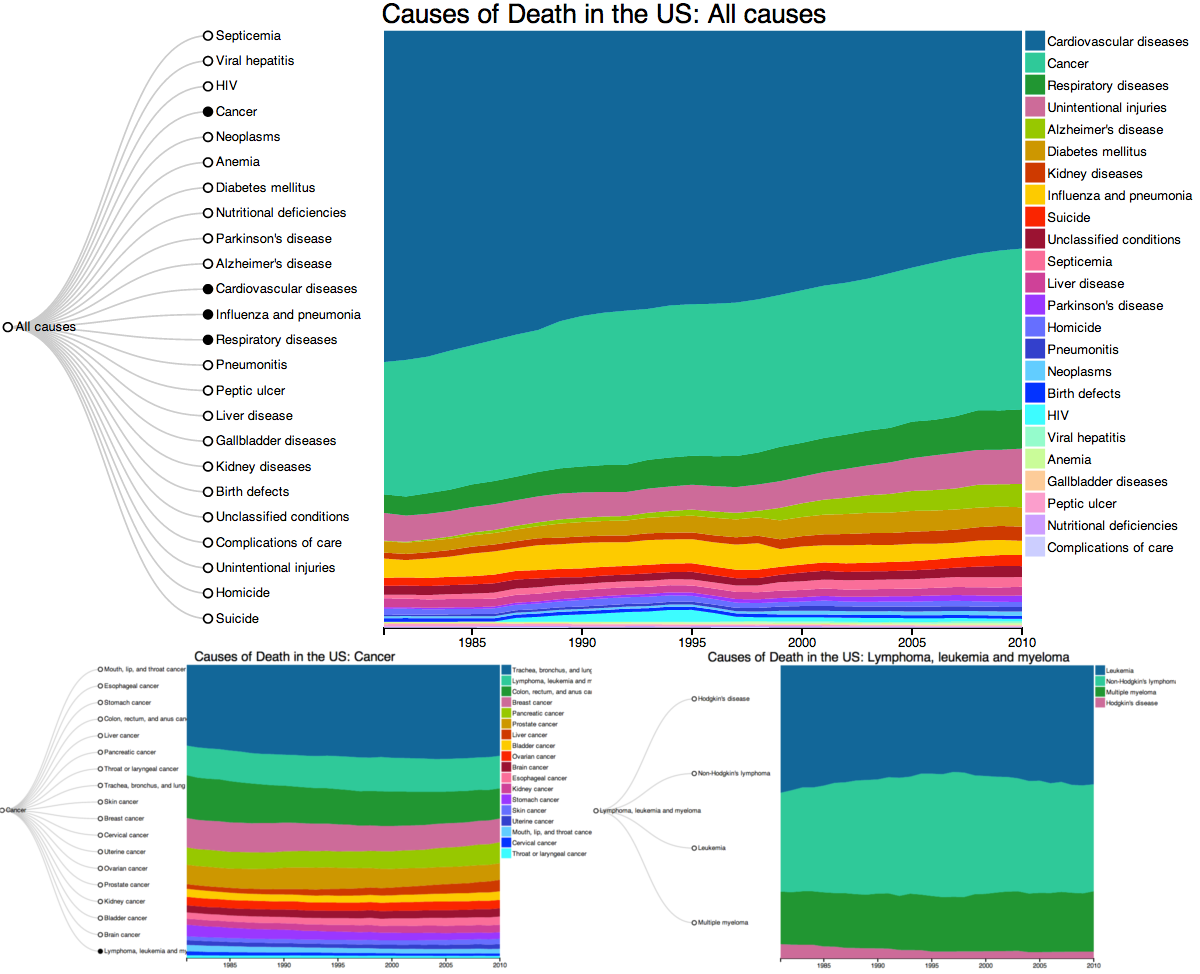
\includegraphics[width=\figureWidth]{figs/mortalityVisV4.png}
  \caption[CDC Mortality Visualization with Linked Views.]
   {Cause of death visualization with two linked views. Navigating up and down the hierarchy by clicking nodes changes the slice of data shown in the stacked area visualization. The top view shows the top-level causes of death. Clicking the ``Cancer'' node yields the view on the bottom left, which shows types of cancer in the stacked area visualization. Further drilling down to ``Lymphoma, leukemia and myeloma'' yields the view on the bottom right.}
  \label{fig:mortalityVisV4}
\end{figure}
\section{Data Set Representation}

In the sections that follow, capitalization denotes terms that have a concrete and well defined meaning within the UDC data structure. These terms include Data Set, Dimension, Member, Measure, Dimension Column, Measure Column, Cube Data Set, Concordance Data Set, Codelist, and Code. Each of these terms will be introduced one by one in terms of what role they play in the UDC data structure. Italicized terms are functions that perform the algorithms associated with data integration and querying. These algorithms operate in terms of the UDC data structure.

A Data Set is a relation with associated metadata that provides context for its interpretation. Tables \ref{table_gdp}, \ref{table_unPop} and \ref{table_concordance} are concrete examples of Data Sets, showing both their relations and metadata. The relation contains the core table of the Data Set. The metadata specifies the interpretation of the relation in terms of Dimensions and Measures. Columns in relations can be annotated in the metadata as either Dimension Columns or Measure Columns. A Dimension Column contains Codes from a single Codelist that refer to Members of a given Dimension. A Measure Column contains numbers representing values for a given Measure. A scaling factor can be associated with each Measure Column to account for varying scales for the same Measure across different Data Sets.

To integrate Data Sets together, we need two kinds of Data Sets, Cube Data Sets and Concordance Data Sets.

\begin{table}
  \caption{A Cube Data Set about Population.}
  \centering
  \label{table_unPop}
  \begin{tabular}{ | c | c | }
    \hline
    table & 
    \begin{tabular}{ | c | c | c | }
      \hline
      \textbf{countryCode} & \textbf{year}& \textbf{pop} \\ \hline
      356 & 1960 & 449595.489 \\ \hline
      356 & 2010 & 1205624.648 \\ \hline
      156 & 1960 & 650680.114 \\ \hline
      156 & 2010 & 1359821.465 \\ \hline
      840 & 1960 & 186361.893 \\ \hline
      840 & 2010 & 312247.116 \\ \hline
    \end{tabular}
    \\ \hline
    dimensions &
    \begin{tabular}{ | c | c | c |}
      \hline
      \textbf{column} & \textbf{dimension} & \textbf{codelist} \\ \hline
      countryCode & Space & UN M.49 \\ \hline
      year & Time & Year \\ \hline
    \end{tabular}
    \\ \hline
    measures & 
    \begin{tabular}{ | c | c | c |}
      \hline
      \textbf{column} & \textbf{measure} & \textbf{scale} \\ \hline
      pop & Population & 1,000 \\ \hline
    \end{tabular}
    \\ \hline
  \end{tabular}
\end{table}

\begin{table}
  \caption{A Cube Data Set about GDP.}
  \centering
  \label{table_gdp}
  \begin{tabular}{ | c | c | }
    \hline
    table & 
      \begin{tabular}{ | c | c | c | }
        \hline
        \textbf{countryCode} & \textbf{year} & \textbf{gdp} \\ \hline
        IND & 1960 & 37679274491.2745 \\ \hline
        IND & 2010 & 1708450861364.17 \\ \hline
        CHN & 1960 & 61377930682.0013 \\ \hline
        CHN & 2010 & 5930529470799.17 \\ \hline
        USA & 1960 & 520531181568 \\ \hline
        USA & 2010 & 14958300000000 \\ \hline
      \end{tabular}
    \\ \hline
    dimensions &
    \begin{tabular}{ | c | c | c |}
      \hline
      \textbf{column} & \textbf{dimension} & \textbf{codelist} \\ \hline
      countryCode & Space & ISO3 \\ \hline
      year & Time & Year \\ \hline
    \end{tabular}
    \\ \hline
    measures & 
    \begin{tabular}{ | c | c | c |}
      \hline
      \textbf{column} & \textbf{measure} & \textbf{scale} \\ \hline
      gdp & Gross Domestic Product & 1 \\ \hline
    \end{tabular}
    \\ \hline
  \end{tabular}
\end{table}

\begin{table}
  \caption{A Concordance Data Set linking equivalent terms used by different cubes referring to countries.}
  \centering
  \label{table_concordance}
  \begin{tabular}{ | c | c | }
    \hline
    table & 
    \begin{tabular}{ | c | c | c | }
      \hline
      \textbf{countryName} & \textbf{unCountryCode}& \textbf{alphaCode} \\ \hline
      India & 356 & IND \\ \hline
      China & 156 & CHN \\ \hline
      United States & 840 & USA \\ \hline
    \end{tabular}
    \\ \hline
    dimensions &
    \begin{tabular}{ | c | c | c |}
      \hline
      \textbf{column} & \textbf{dimension} & \textbf{codelist} \\ \hline
      countryName & Space & UN Geoname \\ \hline
      unCountryCode & Space & UN M.49 \\ \hline
      alphaCode & Space & ISO3 \\ \hline
    \end{tabular}
    \\ \hline
  \end{tabular}
\end{table}

A Cube Data Set contains a relation that represents a data cube using a star schema. Certain columns represent categorical Dimensions, while others represent quantitative Measures. Dimensions are sets of distinct entities that may be unordered, ordered, or hierarchical. Each distinct entity of a Dimension is called a Member. A row in the relation of a Cube Data Set represents a unique set of Members, one from each Dimension of the Cube Data Set, in its Dimension Columns. The unique set of Members represented in each row is called a Cell, which acts like an address in the data cube. Measures are aggregated quantitative properties that can be assigned to Cells in the Measure Columns of the relation. A Cube Data Set contains a set of Observations that draw from a common set of Dimensions and Measures. An Observation links a Cell with concrete values for each Measure. Each complete row of the relation represents a single Observation. Many Cubes can reference the same Dimensions, Members, Cells, and Measures, whereas each Observation belongs to exactly one Cube. Table \ref{table_concepts} provides examples for each of the concepts introduced.

\begin{landscape}
  \begin{table*}
    \caption{Examples for UDC Concepts.}
    \small
    \centering
    \label{table_concepts}
    \begin{tabular}{ | c | c | c |}
      \hline
      \textbf{Concept} & \textbf{Example(s)} & \textbf{Description} \\ \hline
      Dimension & Space, Time & A hierarchy of entities, identified by a string name.\\ \hline
      Measure & Population, Gross Domestic Product & A kind of numeric value that can be\\
              &                                    & assigned to Cells by Observations.\\ \hline
      Cube & The population of India in 1970 was 555.2 million & A set of Observations that draw from \\
           & The population of India in 2010 was 1.206 billion & a common set of Dimensions and Measures. \\
           & The population of China in 1970 was 818.3 million & \\
           & The population of China in 2010 was 1.338 billion & \\ \hline
      Observation & The population of India in 1970 was 555.2 million. & An object that represents a mapping from a Cell \\
      & & to a numeric value for a specific Measure.  \\ \hline
      Cell & India in 1970, China in 2010 & A unique set of Members. \\ \hline
      Member & India, China, 1970, 2010 & A single entity within a Dimension hierarchy, \\
      & & identified by a Code. \\ \hline
      Codelist & Country Name, Country Code & A controlled vocabulary for identifying Members. \\ \hline
      Code & India, in & A single string identifier within a Codelist \\
           &           & that identifies a particular Member. \\ \hline
      Concordance & 
        \begin{tabular}{ c c }
          \textbf{Country Name} & \textbf{Country Code} \\
          India & in \\
          China & cn
        \end{tabular}
      & A relation that defines equivalences between Codes. \\ \hline
    \end{tabular}
  \end{table*}
\end{landscape}

A Member is a unique entity within a Dimension, identified by a single Code. Codelists are controlled vocabularies for referring to Members. A Code is a string within a Codelist that refers to a specific Member. Each Codelist contains Codes that refer to Members of a single Dimension. The metadata of a Cube Data Set defines how some columns of the relation can be interpreted as Dimensions. This metadata is used for transforming the strings in each row of Dimension Columns into Member instances within the UDC data structure.

The Logical Data Structure (LDS) shown in figure \ref{fig_lds} expresses the essential concepts of the UDC data structure and their relationships. This data structure is used to represent Cube Data Sets after they are loaded into memory. Cube Data Sets loaded into this data structure can be integrated together and queried for interactive visualization.
%
%When we read the LDS in figure \ref{fig_lds} according to the rigorous definition described in \cite{carlis2000mastering}, it yields the following assertions:
%%\renewcommand{\theenumi}{\alph{enumi}}
%%\begin{enumerate}
%
%\begin{itemize}
%\item About each Cube we can remember its Dimensions, its Measures, and its Observations.
%\item About each Dimension we can remember its name, its Members, and its Cubes.
%\item About each Measure we can remember its name and its Cubes.
%\item About each Member we can remember its Dimension, its codelist, and its code.
%\item Each Cell is identified by a unique set of Members.
%\item About each Cell we can remember its Members and its Observations.
%\item Each Observation is identified by the combination of its Cube and its Cell.
%\item About each Observation we can remember its values (an object that stores numeric values for each Measure).
%\end{itemize}
%
\begin{figure}
  \centering
  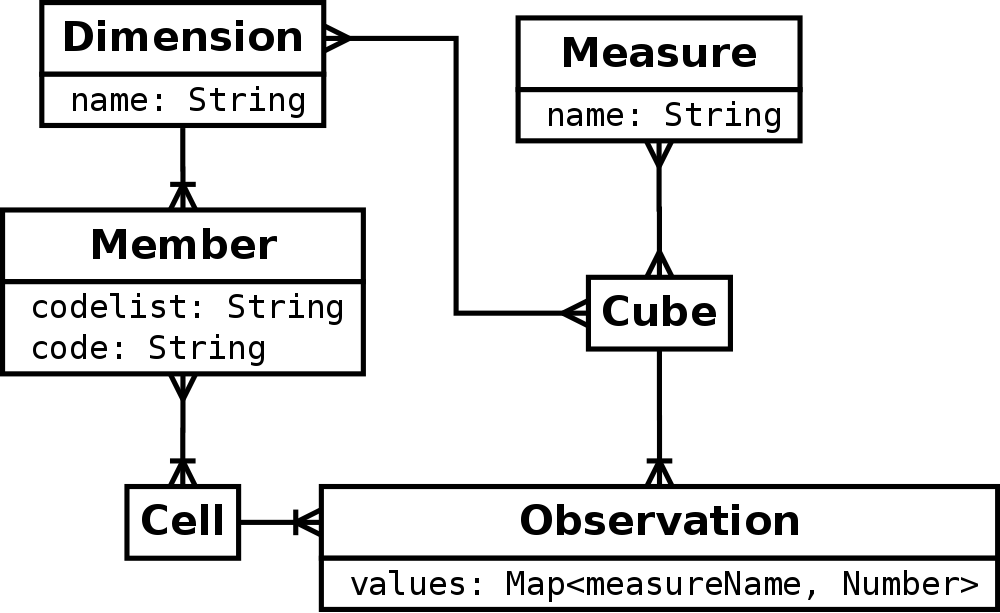
\includegraphics[width=4in]{figs/lds.png}
  \caption [UDC Logical Data Structure]{The Logical Data Structure expressing the representation of Cube Data Sets within the UDC data structure, using the visual data modeling language described in \cite{carlis2000mastering}.}
  \label{fig_lds}
\end{figure}

The following functions transform Data Sets into in-memory representations and help integrate multiple Cube Data Sets together.

\begin{itemize}
\item $createCube(dataset) \rightarrow cube$
\item $createThesaurus(datasets) \rightarrow thesaurus$
\end{itemize}

The $createCube$ algorithm creates a Cube (from figure \ref{fig_lds}) from a Cube Data Set. This procedure must iterate through each Dimension Column and Measure Column of the Data Set to compute the Dimensions and Measures associated with the Cube. Once the metadata has been processed, each row in the relation of the Data Set is transformed into a single Observation. In computing Observations, the requisite Members and Cells are also defined within the in-memory data structure.

The $createThesaurus$ function generates an index that can be used to implement the $canonicalizeMember$ function necessary for merging Cubes. The set of Data Sets input to the $createThesaurus$ function should each be a Concordance Data Set. This means they each have only Dimension Columns that refer to Members of the same Dimension using different Codelists. The relations of Concordance Data Sets serve only to define equivalences between Codes from different Codelists that refer to the same Member. These relations are transformed into an index that maps each $(code, codelist)$ pair to a set of other $(code, codelist)$ pairs that refer to the same Member. The index of equivalence classes can be used in conjunction with a canonical Codelist for each Dimension to implement the $canonicalizeMember$ function. A canonical Codelist can be chosen by sorting all Codelists used in a given Dimension alphabetically and choosing the first one.

\section{Querying Data Sets}
Cubes can be queried by interactive visualizations. Interactive data visualizations need to make a number of different queries for generating user interface components, labels, axes, scales, and visual marks. We assume that a visualization has access to a single Cube containing the integrated data. Starting from the Cube object the following functions provide all queries necessary for general purpose interactive visualizations to operate. This syntax represents functions in terms of their name (before parentheses), what they accept as input (in parentheses), and what they yield as output (after the arrow). Types are denoted as lower case counterparts to UDC concepts, because they represent concrete instances of those concepts.

\begin{itemize}
\item $listDimensions(cube) \rightarrow [dimension]$
\item $listMeasures(cube) \rightarrow [measure]$
\item $listObservations(cube) \rightarrow [observation]$
\item $getValue(observation, measure) \rightarrow \mathbb{R}$
\item $getCell(observation) \rightarrow cell$
\item $member(cell, dimension) \rightarrow member$
\item $slice(cube, cell) \rightarrow cube$
\end{itemize}

The $listDimensions$, $listMeasures$ and $listObservations$ functions list which Dimensions, Measures, and Observations, respectively, are associated with the given Cube. The $getValue$ procedure extracts the numeric value for a given Measure from a given Observation, by evaluating its $values$ property (which maps Measures to numeric values). The $getCell$ procedure reads from the data structure which Cell is associated with the given Observation. The $member$ procedure extracts from the data structure which Member is contained within the given Cell for the given Dimension. The $slice$ procedure implements the traditional OLAP slice operation defined in \cite{datta1999cube}. 

\section{Integrating Data Sets}

The following procedures relate to integrating Cubes:
\begin{itemize}
\item $canonicalizeMember(thesaurus, member) \rightarrow member$
\item $canonicalizeCube(thesaurus, cube) \rightarrow cube$
\item $mergeCubes(cube, cube) \rightarrow cube$
\item $integrate(datasets) \rightarrow cube$ 
\end{itemize}

The $canonicalizeCube$ function transforms a Cube such that all of its Observations use canonicalized Members. When two Data Sets use different Codes to refer to the same Members, the Cubes generated directly from the Data Sets define their Observation domains (Cells) in terms of different Members. A Thesaurus can be used to implement the $canonicalizeMember$ procedure, which resolves equivalent Members referred to using Codes from different Codelists. The $canonicalizeCube$ function invokes $canonicalizeMember$ as a subroutine to normalize the Observations of the Cube. After running $canonicalizeCube$ on two Cubes that use different Codelists, both resulting Cubes use the same Codes to refer to the same Members. This step enables the two Cubes to be merged using $mergeCubes$.

The $mergeCubes$ procedure joins the Observations from two Cubes by matching on their Cells. Each Cell is identified by a unique set of Members. Cells from both Cubes match because the $canonicalizeCube$ procedure was invoked previously on each input cube. In implementing $mergeCubes$, one could employ an inner join strategy, which would yield a Cube with no missing data but may not include all of the original data, or an outer join strategy, which would yield a Cube with missing data (Observations with missing values for some Measures) but would include all of the original data.

Figure \ref{fig:integration} shows the \emph{integrate} algorithm for integrating many Data Sets. This algorithm first transforms all Cube Data Sets in the input $datasets$ array into Cubes using $createCube$, and constructs a Thesaurus from all Concordance Data Sets in the input $datasets$ array using $createThesaurus$. A map-reduce pattern is then applied to integrate all Cubes. The map portion of the algorithm applies the $canonicalizeCube$ function to all Cubes, using the already created Thesaurus to canonicalize Members used in each Cube. The reduce portion of the algorithm applies the $mergeCubes$ function to merge all canonicalized Cubes recursively. The result from the entire algorithm is a Cube that contains data from all of the input Cubes combined and integrated properly. The resulting Cube is suitable for input into interactive visualizations.

\begin{figure}
  \centering
  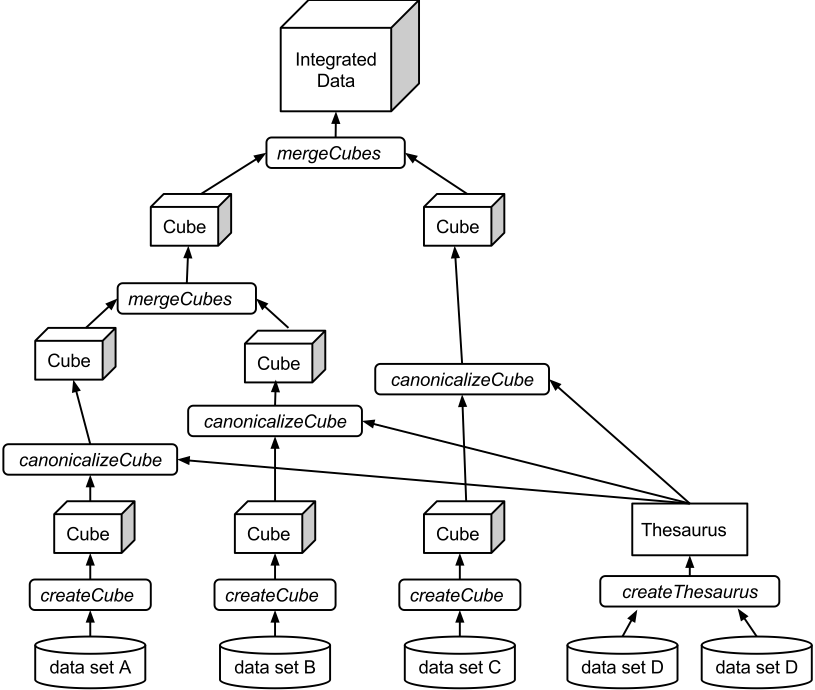
\includegraphics[width=\figureWidth]{figs/integration.png}
  \caption [UDC Data Integration Algorithm]{The flow of the $integrate$ algorithm for integrating data.}
  \label{fig:integration}
\end{figure}

\section{Limitations of Data Cube Representation}
Many, but not all, data sets can be modeled as data cubes. Since data cubes are only capable of representing data that has been aggregated along categorical dimensions, there are many classes of data that do not fit within the conceptual framework of data cubes. For example, a database containing the details of transactions in a supermarket would not be appropriate to model as a data cube. Each entry of a customer purchase may contain a listing of items purchased, how it was paid for, and the date and time the purchase was made. This kind of data fits well into the relational model, but is not appropriate to model as a data cube. Data cubes represent only aggregated summaries, not individual events. In the case of grocery store database containing the transactions for many grocery stores in different regions, while the individual transaction entries cannot be modeled as a data cube directly, a data cube can be constructed from the transactional data by aggregating measures such as ``amount paid'' and ``number of items purchased'' along dimensions such as ``time'', ``region'' and ``product category''. This is a typical data warehouse scenario, where a business aggregates transactional data into a data cube in order to analyze company activities in a summary view.

The key characteristics that allow a given data set to be modeled as a data cube are as follows:

\begin{itemize}
\item The data set contains numeric fields that represent aggregated summaries using sum, average, or some other aggregation operator (measures).
\item The measures of the data set are aggregated along one or more sets of discrete categories or entities (dimensions).
\end{itemize}

Dimensions can be either unordered, ordered, or hierarchical. Dimensions include Space, defining hierarchies of geospatial regions, Time, defining intervals in time, or of any arbitrary collection of categories. Examples of dimensions other than Time and Space include Gender, Ethnicity, and Industry. The Space dimension can be decomposed using several alternative strategies. The most common spatial decomposition found in data is along geopolitical boundaries. Another way to decompose spatial regions is according to a quadrilateralized spherical cube, also called a quad sphere \cite{tobler1986quadtree}. The quad sphere approach provides uniformly distributed regions at multiple levels of detail, which makes it appropriate for presenting aggregated summaries of more detailed data such as billions of points on Earth or satellite imagery data \cite{white1992quadrilateralized}. Yet another alternative geospatial partitioning strategy is by global river basins. Partitioning data by river basins makes sense for climate and weather related data \cite{worldbank2014climate}.

Data sets that have the following qualities may not be modeled directly as data cubes.
\begin{itemize}
\item The data set represents a graph. Graph data such as social network connections or links between Web pages is not supported by the data cube model.
\item The data set contains relational data with a one-to-many relation. For example, a database of transactions in a grocery store where one transaction has many items. Items containing lists of other items cannot be represented using the data cube model. However, one may consider transforming data sets like this such that the nested lists are summarized by some measures (such as total cost or number of items) so the data cube model can be applied.
\item The data set contains entries for individual discrete events or transactions. Data sets with this quality cannot be modeled directly as data cubes, however it may be possible to compute data cubes by aggregating them using OLAP techniques from data warehousing.
\end{itemize}

Although data sets with the above qualities may not be modeled directly as data cubes, it may be possible to compute data cubes that summarize data sets like these. For example, the BrightKite data set which was originally structured as a graph \cite{cho2011friendship} can be aggregated using the data cube approach then visually analyzed \cite{liu2014effects, liu2013immens}. Any graph data set in which nodes contain metadata such as location and time can be aggregated along Space, Time and other dimensions to form a data cube.

\section{Proof of Concept}

The United Nations (UN) Population Prospects Data Set provides population data for each country of the World over time. A small sample of this data set is shown in table \ref{table_unPop}. This data set was downloaded as an Excel spreadsheet (shown in figure \ref{fig:unPopExcel}), exported as a Comma Separated Value (CSV) file, then transformed to be in the format expected by a data cube dataset (one row for each Observation). This data set uses the UN M.49 country codes to refer to countries. Figure \ref{fig:unTimeline} shows a slice of this data set showing population values over time for the entire world. This visualization gives a broad overview of the data. By drilling down, lines in the line chart can be made to represent individual countries.

\begin{figure}
  \centering
  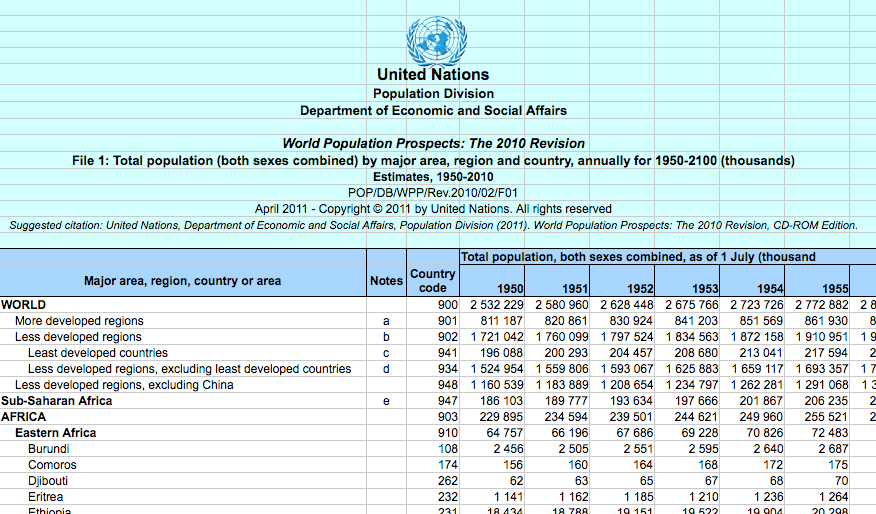
\includegraphics[width=\figureWidth]{figs/UN_World_Population_Spreadsheet.png}
  \caption [United Nations Population Prospects Data Set]{The United Nations Population Prospects data set \cite{unPopData}, made available in Excel format. This is an example data set that can be imported into our data structure and integrated with other data sets.}
  \label{fig:unPopExcel}
\end{figure}

\begin{figure}
  \centering
  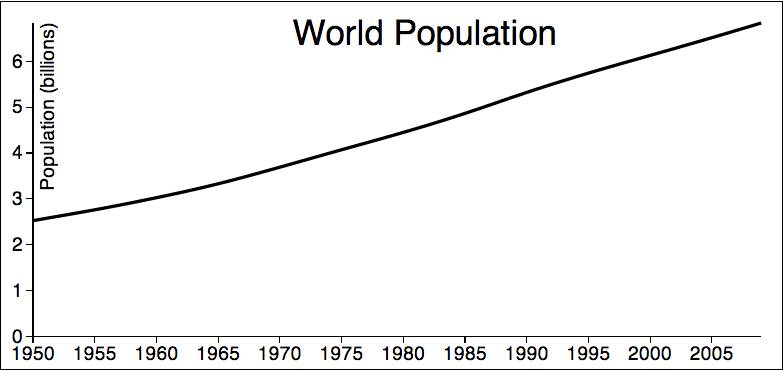
\includegraphics[width=\figureWidth]{figs/unTimeline.png}
  \caption [World Population Timeline]{A timeline visualization of the United Nations Population Estimates data set. This shows the population of the entire world from 1950 to 2010.}
  \label{fig:unTimeline}
\end{figure}

The World Bank publishes publicly available data about a number of topics. One dataset from the World Bank contains the Gross Domestic Product (GDP) of each country over many years, shown in figure \ref{fig:worldBankGDP}. A small sample of this data set is shown in table \ref{table_gdp}. This data set uses the ISO3 standard Codelist for countries.

\begin{figure}
  \centering
  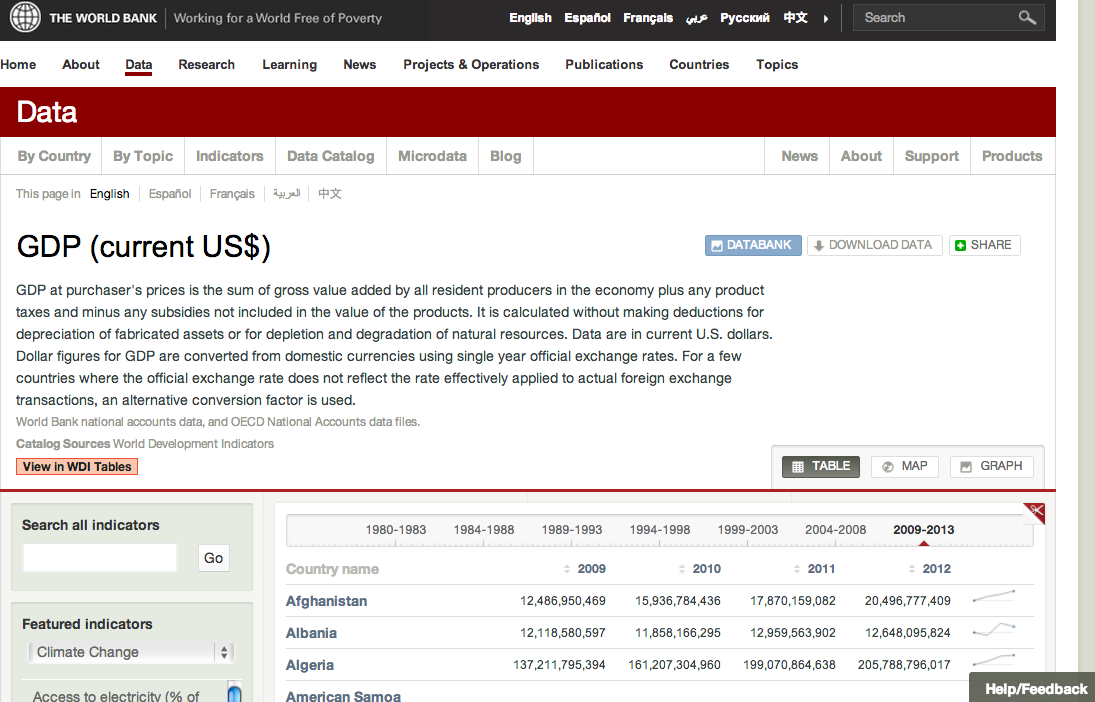
\includegraphics[width=\figureWidth]{figs/worldBankGDP.png}
  \caption[World Bank GDP Data Set]{The World Bank GDP Data Set.}
  \label{fig:worldBankGDP}
\end{figure}

We applied the UDC approach to modeling and integrating the UN Population Prospects data set and the World Bank GDP data set. The resulting integrated Cube was visualized as a scatter plot, shown in figure \ref{fig:scatter}. In this visualization, Population is mapped to the X axis, GDP is mapped to the Y axis, and each dot represents a country. Both axes are log normalized in order to spread the data. This plot shows that there is a correlation between Population and GDP, and that both measures follow roughly a Power Law distribution. This demonstrates a proof of concept implementation of the UDC data structure and algorithms for integrating and visualizing public data.

Consider the steps required to produce the scatter plot visualization of the integrated Population and GDP Cube shown in figure \ref{fig:scatter}. First, the dimensions of the integrated Cube, namely Time (Years) and Space (Countries), can be computed using the $listDimensions$ function. Since we want each dot to represent a country, the Cube must then be sliced using the $slice$ function such that it contains only data for a single year. Next, the X and Y scales must be defined. The $listMeasures$ procedure can be used to generate a list from which users can choose which measures to assign to the X and Y axes. Once X and Y measures are chosen, the $listObservations$ procedure can generate the list of Observations to transform into visual marks (one for each Country). To compute the domains for the X and Y scales, the Observations can be queried for their X and Y measure values using the $getValue$ procedure. The minimum and maximum values returned for the X and Y measures can define the domains for the X and Y scales. Once the scales have been defined, the Observations can be iterated over once more to generate the complete visualization. This is one example of how the given query algorithms for Cube Data Sets can be used for visualization. 

\begin{figure}
  \centering
  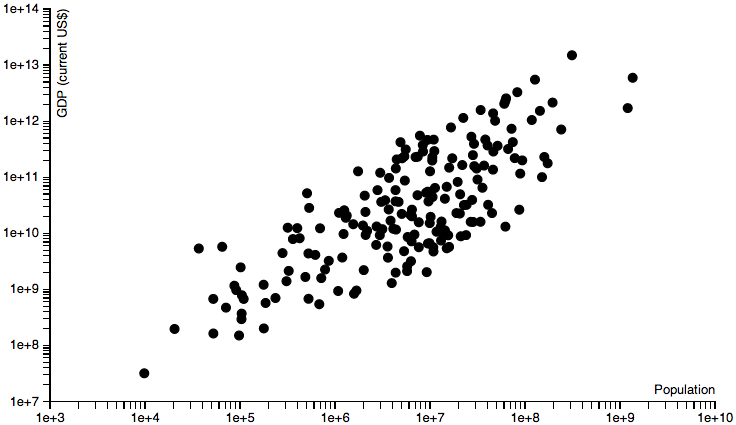
\includegraphics[width=\figureWidth]{figs/scatter.png}
  \caption[Scatter Plot of Integrated Data]{A scatter plot visualizing two data sets integrated together. The X axis shows Population, drawn from a United Nations data set, and the Y axis shows GDP, drawn from a World Bank data set. Each dot represents a country.}
  \label{fig:scatter}
\end{figure}

The $slice$ procedure can be utilized for developing visualizations with multiple linked views. This is when one visualization shows an overview, and interactions in that visualization can define how the input data for another visualization is sliced before it is visualized. We have implemented a prototype of this concept which uses a linked Choropleth Map and Line Chart, shown in figure \ref{fig:choropleth}. Zooming in the Choropleth Map defines the set of countries represented as lines in the Line Chart. Selecting a year in the Line Chart causes the Choropleth Map to show data for that year only.

\begin{figure}
  \centering
  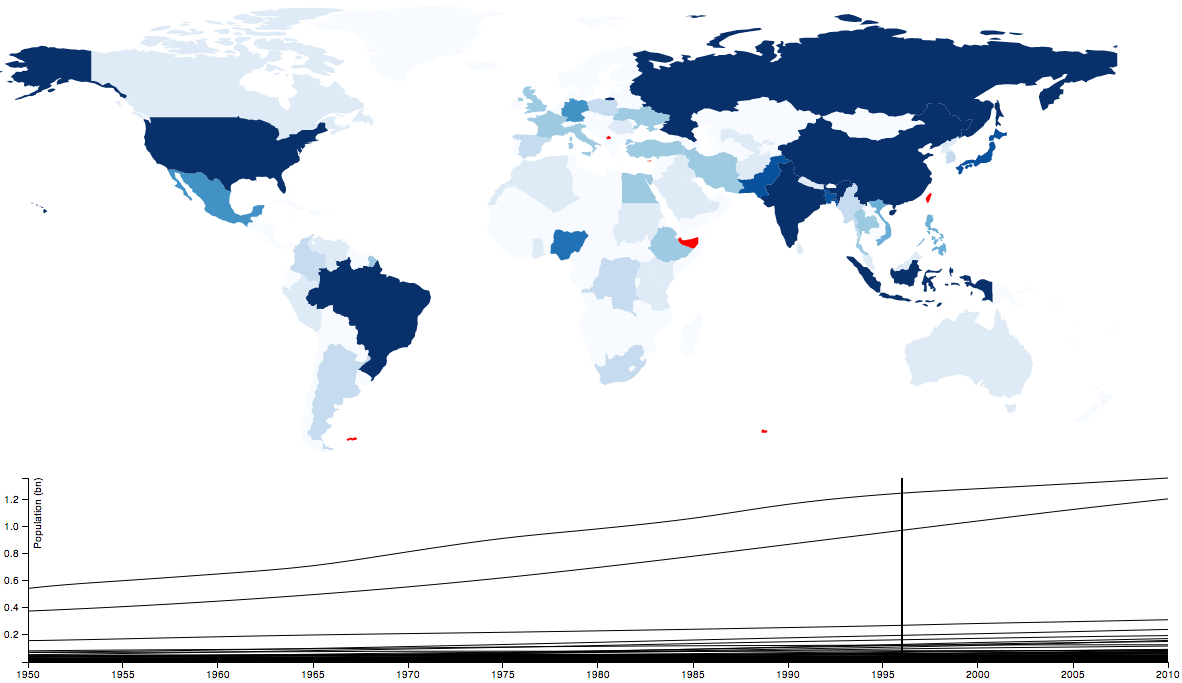
\includegraphics[width=\figureWidth]{figs/choropleth.png}
  \caption [Linked Line Chart and Choropleth Map]{A linked line chart and Choropleth map showing population data from the United Nations. Zooming in the map filters the line chart. Selecting a year in the line chart causes the map to show data from that year. This demonstrates how the $slice$ procedure can be utilized for generating interactive visualizations with linked views. Red indicates missing data.}
  \label{fig:choropleth}
\end{figure}

\section{Crowdsourcing Data Experiment}
Rather than manually curating data, a crowdsourcing approach can be taken to data collection for the UDC. We have performed an initial experiment to test the feasibility of this approach. Amazon Mechanical Turk supports assignment of tasks, called ``Human Intelligence Tasks'' or HITs, to workers who get paid small amounts (on the order of cents) to execute the tasks. To populate the UDC using Mechanical Turk, HITs can be devised that ask workers to find an answer to a simple question like ``What was the population of India in 1950?''. This question is an instance of a more general form ``What was the \verb1${measure}1 of \verb1${place}1 in \verb1${time}1''. By enumerating possible values for \verb1${measure}1, \verb1${place}1, and \verb1${time}1, responses to such HITs can populate large regions of the UDC.

To test the crowdsourcing data collection approach, an experiment was performed using Amazon Mechanical Turk. In this experiment, \verb1${measure}1 = population, \verb1${place}1 = \{India, China, United States\}, and \verb1${time}1 = \{1950, 2010\}. The results contained between 7 and 10 responses from multiple workers for each combination of place and time. By taking the mode (most frequently occurring value) of the worker submissions for each combination of place and time, the following table was generated:

\begin{figure}[h!]
  \centering
  \begin{tabular}{ | l | l | l | l | }
  \hline
  Place & Time & Population & Source URL \\ \hline
  India & 1950 & 369880000 & \tiny \verb1www.geohive.com/earth/population3.aspx1 \\ \hline
  China & 1950 & 563000000 & \tiny \verb1geography.about.com/od/populationgeography/a/chinapopulation.htm1 \\ \hline
  USA & 1950 & 150697361 & \tiny \verb2en.wikipedia.org/wiki/1950_United_States_Census2 \\ \hline
  India & 2010 & 1150000000 & \tiny \verb1www.indiaonlinepages.com/population/india-population.html1\\ \hline
  China & 2010 & 1339724852 & \tiny \verb1en.wikipedia.org/wiki/Demographics_of_China1\\ \hline
  USA & 2010 & 308745538 & \tiny \verb1en.wikipedia.org/wiki/United_States_Census1\\ \hline
  \end{tabular}
  \caption[Mechanical Turk Results]
   {Initial results from an experiment in crowdsourcing public data using Amazon Mechanical Turk.}
  \label{fig:crowdData}
\end{figure}

In the table shown in figure \ref{fig:crowdData}, each row represents an observation within the data cube. The values in the Place column refer to members of the Space dimension. The values in the Time column refer to members of the Time dimension. The values in the Population column assign numeric values to cells (combinations of Space and Time members) for the Population measure. This initial result demonstrates the feasibility of crowdsourced data collection for the UDC.

\section{Summary}
This chapter introduced novel data structures and algorithms for integration of multiple data sets, and for querying the merged data structure for use in interactive visualizations. We call this collection of data structures and algorithms the Universal Data Cube (UDC). This approach functions by using concordances to canonicalize identifiers used across data sets, then merging data cubes in a map-reduce fashion. The resulting integrated structure can be queried for generation of interactive visualizations. Future work will focus on developing reusable interactive visualizations that can use the UDC data structure as input, and on a framework for easily assembling linked views based on the UDC data structure.

